\documentclass[a4paper, 12pt]{article}%тип документа

%отступы
\usepackage[left=2cm,right=2cm,top=2cm,bottom=3cm,bindingoffset=0cm]{geometry}

%Русский язык
\usepackage[T2A]{fontenc} %кодировка
\usepackage[utf8]{inputenc} %кодировка исходного кода
\usepackage[english,russian]{babel} %локализация и переносы

%Вставка картинок
\usepackage{wrapfig}
\usepackage{graphicx}
\graphicspath{{pictures/}}
\DeclareGraphicsExtensions{.pdf,.png,.jpg}
\usepackage{subcaption,floatrow,graphicx,calc}

\DeclareFloatSeparators{mysep}{\hspace{1cm}}

%оглавление
\usepackage{titlesec}
\titlespacing{\chapter}{0pt}{-30pt}{12pt}
\titlespacing{\section}{\parindent}{5mm}{5mm}
\titlespacing{\subsection}{\parindent}{5mm}{5mm}
\usepackage{setspace}

%Графики
\usepackage{multirow}
\usepackage{pgfplots}
\pgfplotsset{compat=1.9}

%Математика
\usepackage{amsmath, amsfonts, amssymb, amsthm, mathtools}

%Стиль страницы
\usepackage{fancyhdr}
\pagestyle{fancy}

\newcommand{\x}{\cdot}

\begin{document}

\begin{titlepage}

\begin{center}
%\vspace*{1cm}
\large\textbf{Московский Физико-Технический Институт}\\
\large\textbf{(государственный университет)}
\vfill
\line(1,0){430}\\[1mm]
\huge\textbf{Работа 5.2.2/5.2.3}\\
\line(1,0){430}\\[1mm]
\vfill
\large Сибгатуллин Булат, ФРКТ\\
\end{center}

\end{titlepage}
\fancyhead[L] {Работа 5.2.2/5.2.3}
\noindent \textbf{Цель работы:} \\
\indent Исследовать спектральные закономерности в оптических спектрах водорода и дейтерия. По резелутатам измерений вычилить постоянные Ридберга для этих двух изотопов водорода, их потенциалы ионизации, изотопические сдвиги линий.
	
	Исследовать спектр поглощения паров йода в видимой области; по результатам измерения вычислить энергию колебательного кванта молекулы йода и энергия её диссоциации в основном и возбужденном состояниях.

\section{Теоретическая часть}
\subsection{Cпектр водорода}
Атом водорода является простейшей квантовой системой, для которой уравнение Шрёдингера может быть решено точно. Это также верно для водородноподобных атомов, то есть атомов с одним электроном на внешней оболочке. Из решения уравнения Шрёдингера следует, что внешний электрон в таких атомах обладает дискретным энергетическим спектром:  
\begin{equation}
	E_n = - \frac{m_e (Z e^2)^2}{2\hbar^2}\frac{1}{n^2},
\end{equation}
где $n$ есть номер энергетического уровня, $Z$ есть зарядовое число ядра рассматриваемого атома, которое в случае атома водорода равно 1.\\
При переходе электрона с $n$-го на $m$-й уровень излучается фотон с энергией
\begin{equation}
	E_\gamma = E_n - E_m = \frac{m_ee^2}{2\hbar^2}Z^2\left(\frac{1}{m^2} - \frac{1}{n^2}\right).
\end{equation}
Длина волны  соответствующего излучения $\lambda_{n,m}$ связана с номерами уровней следующим соотношением:
\begin{equation}
	\label{eq:Ry}
	\lambda_{n,m}^{-1} =\frac{m_ee^2}{4\pi\hbar^3c}Z^2\left(\frac{1}{m^2}-\frac{1}{n^2}\right) = \text{Ry} Z^2 \left(\frac{1}{m^2}-\frac{1}{n^2}\right),
\end{equation}
где $\text{Ry} = \frac{m_ee^2}{4\pi\hbar^3c}$ есть постоянная Ридберга.

В данной работе будет исследоваться серия Бальмера атома водорода, в которой электроны совершают переходы с некоторого уровня $n$ на уровень $m = 2$.
\subsection{Cпектр йода}
В первом приближении энергия молекулы может быть представлена в виде:
\begin{equation}
	E=E_e+E_o+E_r,
\end{equation}
где $E_e$ есть энергия электронных уровней, $E_o$ есть энергия колебательньных уровней, $E_r$ есть энергия вращательных уровней.

В настоящей работе рассматриваются оптические переходы, то есть переходы, связанные с излучением фотонов в видимом диапазоне длин волн. Они соответсвтуют переходам между различными электронными состояниями. При этом также происходят изменения вращательного и колебательного состояний, однако в реальности ввиду малости характерных энергий вращательные переходы ненаблюдаемы.

Более конкретно, изучаются переходы из колебательного состояния с номером $n_1$ освновного электронного уровня с энергией $E_1$ в колебательное состояние с номером $n_2$ на электронный уровень с энергией $E_2$. Энергия таких переходов описывается формулой:
\begin{equation}\label{iod}
	h \nu_{n_1,n_2}=(E_2-E_1)+h\nu_2(n_2+\dfrac{1}{2})-h \nu_1(n_1+\dfrac{1}{2}),
\end{equation}
где $\nu_1$ и $\nu_2$ суть энергии колебательных квантов на электронных уровнях с энергиями $E_1$ и $E_2$.

При достаточно больших квантовых числах $n_1$ и $n_2$ колебательные уровни переходят в непрерывный спектр, что соответствует диссоциации молекулы. Наименьшая энергия, которую нужно сообщить молекуле в нижайшем колебательном состоянии, чтобы она диссоциировала, называется энергией диссоциации.

В данной работе определяются энергии диссоциации на первых двух электронных уровнях.
	
\section{Экспериментальная установка}
	Для измерения длин волн спектральных линий в работе используется стеклянный-призменный монохроматор-спектрометр УМ-2 (универсальный монохроматор), предназначенный для спектральных исследований в диапазоне от 0,38 до 1,00 мкм. Основные элементы монохроматора представлены на \ref{pic1}.
	\thisfloatsetup{floatrowsep=mysep}	
	\begin{figure}[h!]
		\ffigbox{
			\begin{subfloatrow}[2]
				\ffigbox[\FBwidth]{\caption{}}%
				{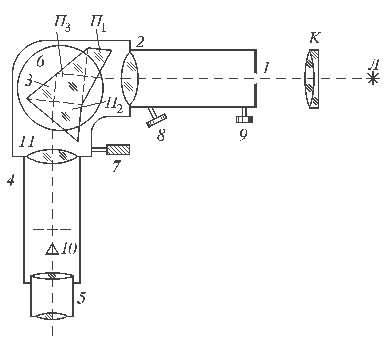
\includegraphics[scale=1]{images/ustanovka1.pdf}{\label{pic1}}}
				\ffigbox[\FBwidth]{\caption{}}%
				{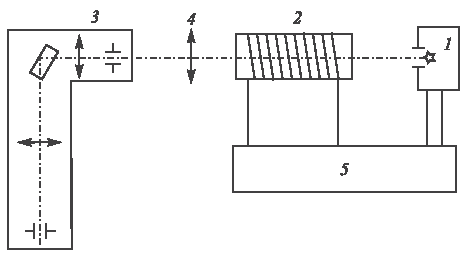
\includegraphics[scale=1]{images/ustanovka2.pdf}{\label{pic2}}}         
			\end{subfloatrow}
		}
		{\caption{Экспериментальная установка.}}
	\end{figure}
	
	В нашей работе спектр поглощения паров йода наблюдается визуально на фоне сплошного спектра лампы накаливания 1, питаемой от блока питания 2 (рис.~\ref{pic2}).

\section{Выполнение работы}

\begin{enumerate}
\item Выполним градуировку монохроматора. Проведем серию измерений для спектра неона и ртути. Данные запишем в таблицу.

\begin{figure}[h!]
\centering
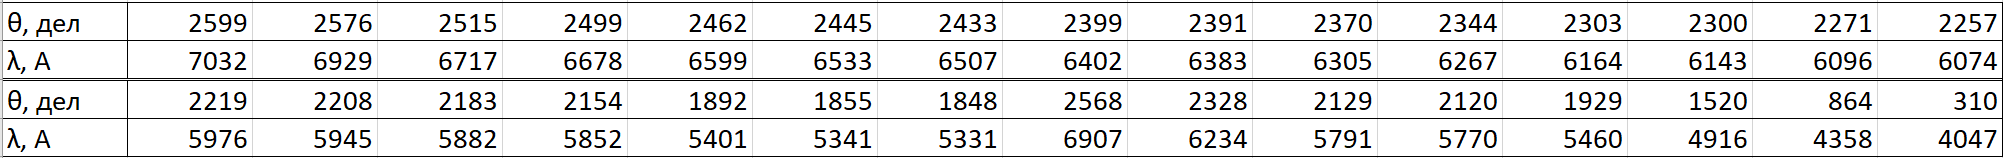
\includegraphics[width = \linewidth]{images/table.png}
\caption{Данные для градуировки монохроматора}
\label{mirror}
\end{figure}

\item Построим график по получившимся данным.

\begin{figure}[h!]
\centering
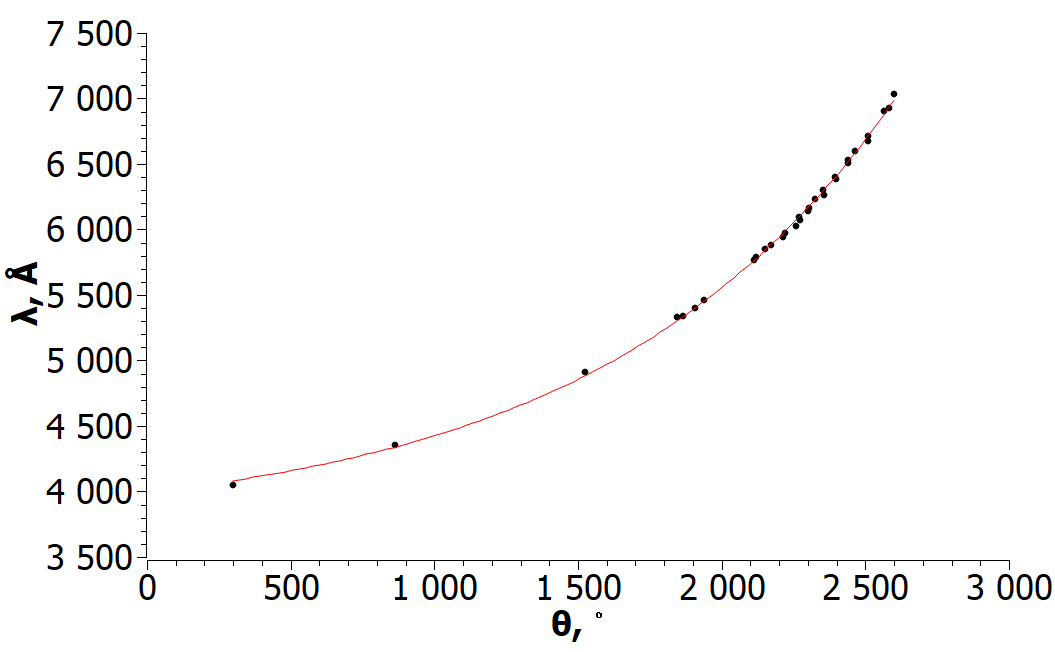
\includegraphics[width = 0.8\linewidth]{images/graph.png}
\caption{График градуировки монохроматора}
\label{mirror}
\end{figure}

Итоговая функция представима в виде:

\[y = a + b\cdot \exp^{x/c}\]

Получаем значения для коэффициентов:

\begin{center}
\begin{tabular}{|c|c|c|}
\hline 
 & Значение & Погрешность \\ 
\hline 
a & 3727 & 36 \\ 
\hline 
b & 267 & 16 \\ 
\hline 
c & 1039 & 2 \\ 
\hline 
\end{tabular} 
\end{center}

Имеем:

\[y = 3727 + 267 \cdot \exp^{x / 1039}\]

\item Проведем измерения для водорода и заодно проверим формулу Бальмера (Таблица \ref{table_mn}):

\begin{table}[h!]
		\caption{Определение линий спектра водорода}
		\begin{center}
			\begin{tabular}{|c|c|c|c|c|c|c|}
				\hline 
				Линия спектра & $ \theta $, $ ^\circ $ & $ \lambda, \;\mathring{A} $ & $ m $ & $ \frac{1}{n^2} - \frac{1}{m^2} $ & $ \frac{1}{\lambda}, \;  10^{-4} \mathring{A}^{-1} $  &  $ \sigma_{\frac{1}{\lambda}}, 10^{-4} \mathring{A}^{-1} $ \\ 
				\hline 
			$ H_\alpha $ & 2452 & 6554 & 3 & 0.139 & 1.528 & 0.092 \\
			\hline
		$ H_\beta $  & 1464 & 4819 & 4 & 0.188 & 2.059 & 0.124 \\
		\hline
			$ H_\gamma $ & 838 & 4325 & 5 & 0.21 & 2.3 & 0.138 \\
			\hline
			$ H_\delta $ & 415 & 4125 & 6 & 0.222 & 2.436 & 0.146 \\
				\hline 
			\end{tabular} 
		\end{center}
		\label{table_mn}
	\end{table}

\item Используем МНК, чтобы проверить, является ли зависимость $\frac{1}{\lambda}(\frac{1}{n^2} - \frac{1}{m^2})$ линейной (проверить формулу Бальмера).

Получим зависимость вида $y = ax + b$:

	\begin{table}[H]
		\begin{center}
			\begin{tabular}{|c|c|c|}
				\hline
				& Значение & Погрешность \\
				\hline
				 $ b $ & 0.0170 & 0.0053 \\
				 \hline
				$ a $& 10.9567 & 0.0276 \\
				\hline 
			\end{tabular} 
		\end{center}
	\end{table}
	
Определим постоянную Ридберга:

\[
R = 108453 \pm 6574 \text{см}^{-1}
\]

\item Перейдем к измерениям спектра молекулы йода. Найдем $\theta_{1,0}, \theta_{1,5}, \theta_{\text{гр}}$:

\begin{itemize}
		\item $ \theta_{1, 0} \approx 2386 \Rightarrow \lambda_{1, 0} \approx 6380 \mathring{A} \Rightarrow \nu_{1, 0} \approx 4,7 \x 10^{14} \; Гц \Rightarrow  h \nu_{1, 0} \approx 1,95 \; эВ $
		
		\item $ \theta_{1, 5} \approx 2282 \Rightarrow \lambda_{1, 5} \approx 6128 \mathring{A} \Rightarrow \nu_{1, 5} \approx 4,9 \x 10^{14} \; Гц \Rightarrow  h \nu_{1, 5} \approx 2,03 \; эВ $
			
		\item $ \theta_{гр} \approx 1616 \Rightarrow \lambda_{гр} \approx 4991 \mathring{A} \Rightarrow \nu_{гр} \approx 6,0 \x 10^{14} \; Гц \Rightarrow  h \nu_{гр} \approx 2,47 \; эВ $
	\end{itemize}
	
Отсюда энергия колебательного кванта возбужденного состояния молекулы йода согласно \eqref{iod}
	
	\begin{equation}\label{}
	h\nu_2 = \dfrac{h\nu_{1, 5} - h\nu_{1, 0}}{5} = 0,0164 \pm 0,0079 \; эВ
	\end{equation}
	
	Вычислим по формуле \eqref{iod} разницу $ E_2 - E_1 = h\nu_{эл}$, сделав сдвиг серии на 1 (вычтя $ h\nu_1 $):
	
	\begin{equation}\label{}
	h \nu_{эл} = h \nu_(1,0) - \dfrac{1}{2} h\nu_2 + \dfrac{3}{2}h\nu_1 \approx 1,98  \pm 0,02 \; эВ
	\end{equation}
	
	Отсюда получаем энергии диссоциации частицы в основном ($ D_1 $) и возбужденном состоянии, считая $ E_a = 0,94 $ эВ:
	
	\section{Вывод}
	
	Мы изучили спектры в оптических спектрах водорода и йода, экспериментально проверили справедливость формулы Бальмера и нашли постоянную Ридберга, которая в пределах погрешность совпадает с табличной ($ R = 109 678 \; см^{-1} $), заметим, что погрешность в большей степени возникает из-за представления зависимости калибровочных данных как функции экспоненты. Этот вклад ($ \approx 6\%$) влияет на погрешность на протяжении всех измерений. Оценили энергии квантов возбужденного состояния молекулы, энергию диссоциации частиц и энергию электронного перехода.

\end{enumerate}

\end{document}